% Chapter 4
\chapter{SYSTEM ARCHITECTURE} % All Chapter headings in ALL CAPS

\section{Global Positioning System}

The GPS module handles collection of the geolocational data and passes this data to the MCU. This module is activated by an interrupt from the MCU which is generated whenever an accident is detected by the MCU. The coordinates are formatted into the Payload format (Refer section \ref{sub:payload}) \\

\includepdf[scale=1.18,pages={1}]{../Figures/final_block.pdf}

\noindent A pseudocode working of the GPS \\

\begin{verbatim}
On Interrupt
begin
     Collect coordinates
     Format coordinates
end interrupt handler
\end{verbatim}

The GPS might not be accurate in closed locations, but on roads, the data provided by GPS will be of high accuracy.

\section{Global System for Mobile Communication}

GSM is a digital mobile telephone system that is widely used in Europe and other parts of the world. The GSM module performs two crucial functions. It receives the payload from the MCU, notifies the emergency services and also transmits the payload to the centralized server.

\begin{verbatim}
if (Payload received)
begin
     Notify Emergency Services
     Send Payload
endif
\end{verbatim}

A small snippet outlining the primary workings of the GSM module.

\noindent\textbf{Notify Emergency Services} \\
\noindent\textbf{Input} : Payload \newline
\textbf{Output} : Result (Success, Error)

\begin{verbatim}
begin
     Get emergency contacts from owner file
     Send payload to the emergency contacts using AT commands
end 
\end{verbatim} 

The ARU contains an owner file which is created when a new user registers. This file contains info about user that is made part of the payload. This payload (\ref{sub:payload}) is sent to the emergency services with the help of AT commands. \\

\noindent\textbf{Send Payload} \\
\noindent\textbf{Input}: AccidentPayload \newline
\textbf{Output} : Log report

\begin{verbatim}
begin
     Send POST request to the server to report new accident
     Include the accidentPayload (in JSON) in the POST request
     Log report if response code is 201
end 
\end{verbatim}

The server accepts a POST request which contains the accident payload. On successful request, it sends a 201 (Content created) response or else returns a 400 (Bad request) upon which, the device schedules a send later. 

\section{Arduino Microcontroller}

An Arduino board is the main module of the system. It detects the accident with the help of the Airbag deployment unit and uses the GPS and GSM modules to do the required work.

\begin{verbatim}
Init GPS module
Init GSM module
while (MCU is running)
     Ping Deployment Unit for Accident SIG
     if (SIG == true)
     begin
          Ping GPS module for coordinates
          Convert to payload format
          Send to GSM
     endif
end while
\end{verbatim}

This code snippet initialises and sets up the Microcontroller unit to respond to accidents. Whenever an accident happens, the MCU gets the coordinates from the GPS module, converts into a format recognised by the server and forwards it to the GSM module.

\subsection{Smartphone application}

We make use of a smart-phone application in case of a false alarm. We can't always rely on air bag deployment as an indicator of some serious accidents. There are instances in which air bags are deployed even for some minor accidents and it is not necessary to notify the emergency services. In those cases, the app provides an option to cancel the alarm (i.e. false alarm). The airbag deployment unit triggers the micro-controller unit as well as activates the mobile application. The mobile app allows the user to interrupt further process in case of a false alarm with a timeout of 2 minutes. The GSM module holds the data during that time out. If the alarm has not been cancelled in that particular timeout then the triggered alarm is considered to be genuine and the process continues. The GSM after the timeout notifies the emergency services and sends the data to web server for analysis.

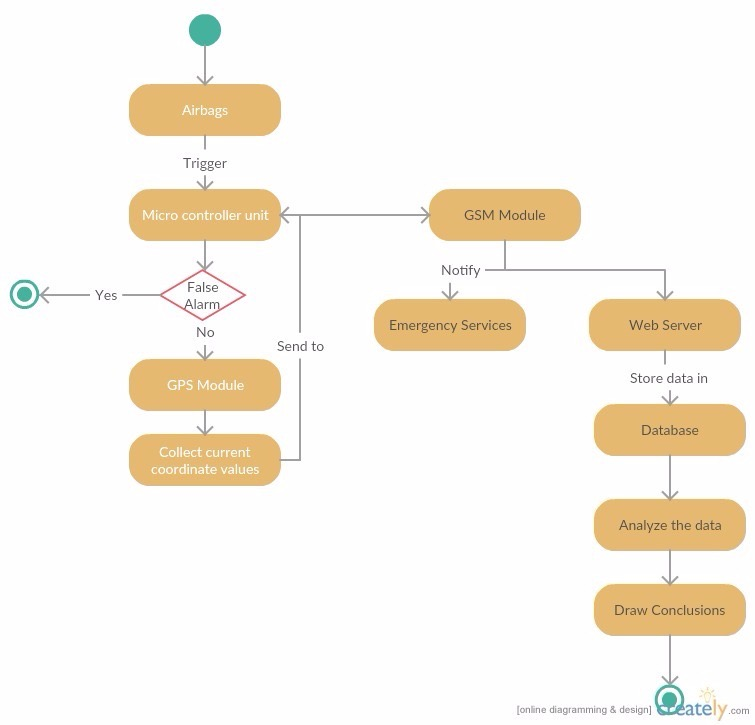
\includepdf[scale=0.85,pages={1}]{../Figures/acti.pdf}

